% -------------------------------------------------------
\subsection*{Analytical Matrix Modeling}
% -------------------------------------------------------

The primary bandwidth bottleneck at the receiver front-end is the lumped parasitic capacitance
contributed by the electrostatic discharge (ESD) protection diodes, the bond pad, and the
receiver input gate. The input network must absorb these parasitics to present a broadband
$50\,\Omega$ impedance at the chip boundary up to the PCIe~Gen~6 Nyquist frequency of 32~GHz,
thereby minimising Inter-Symbol Interference (ISI) due to impedance mismatch.

\vspace{\baselineskip}

To predict the high-frequency behaviour of the network analytically, a cascaded ABCD-matrix
model was developed in MATLAB. The T-coil core was first described by its ABCD parameters.
To correctly account for the bridging capacitance~$C_b$, which appears in parallel across the
two-port rather than in series with it, the core ABCD matrix was converted to its equivalent
admittance (Y-matrix) representation. The shunt admittance of~$C_b$ was then added directly,
and the combined matrix was transformed back into ABCD form. This formulation yields an exact
fifth-order closed-form transfer function for the complete network, which was subsequently
used to extract $Z_{in}$, $S_{11}$, and the system pole-zero map.

\vspace{\baselineskip}

The model was used to tune the component values with the objective of maintaining
$\text{Re}\{Z_{in}\} = 50\,\Omega$ over the widest achievable bandwidth. Specifically,
the optimisation target was to keep the real impedance within the $40\,\Omega$ to $60\,\Omega$
tolerance window mandated by the PCIe~sig specification for a 64~GT/s link.
The analytical performance of the optimised network is presented in
Figure~\ref{fig:matlab_analysis}, and the resulting target design values are summarised in
Table~\ref{tab:target_values}. The schematic used as the basis for the matrix model is shown
in Figure~\ref{fig:model_schematic}.

\vspace{1cm}
\begin{figure}[H]
    \centering
    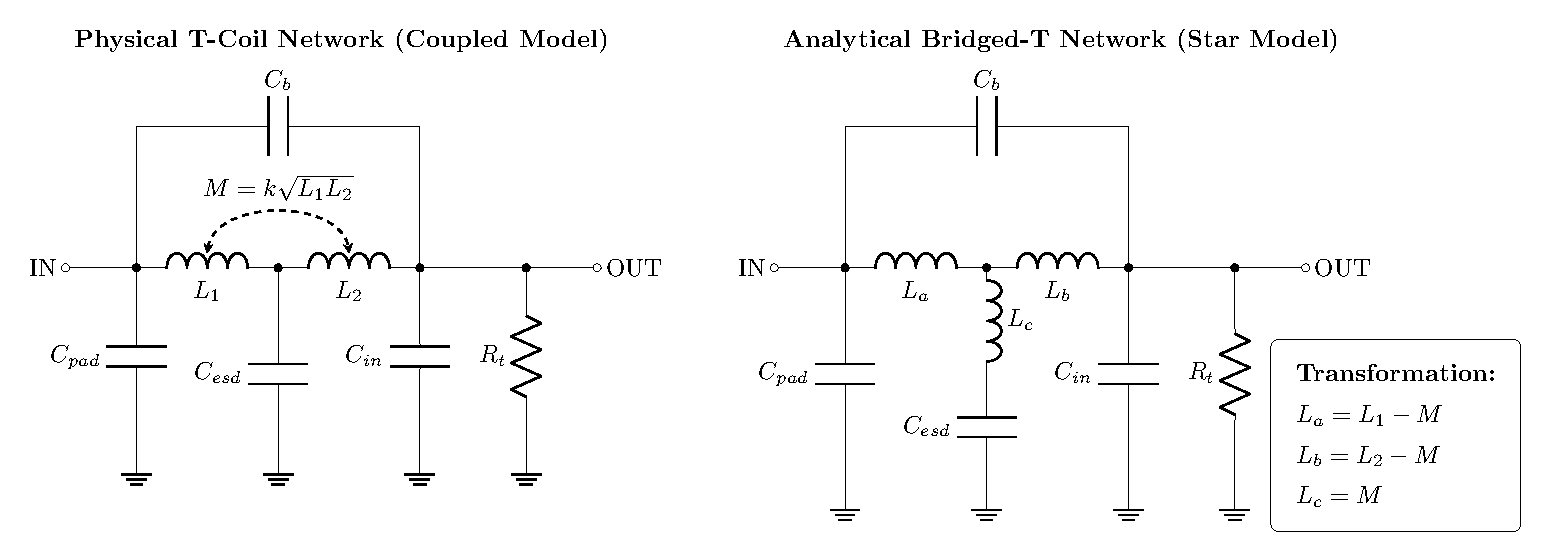
\includegraphics[width=\linewidth]{img/Termination_VGA_img/matlab_model.pdf}
    \caption{Used model for the cascaded ABCD matrix formulation.}
    \label{fig:model_schematic}
\end{figure}

% --- 4-panel MATLAB figure: stacked 1x4 ---
\begin{figure}[H]
    \centering

    % --- First Row ---
    \begin{subfigure}[b]{0.48\textwidth}
        \centering
        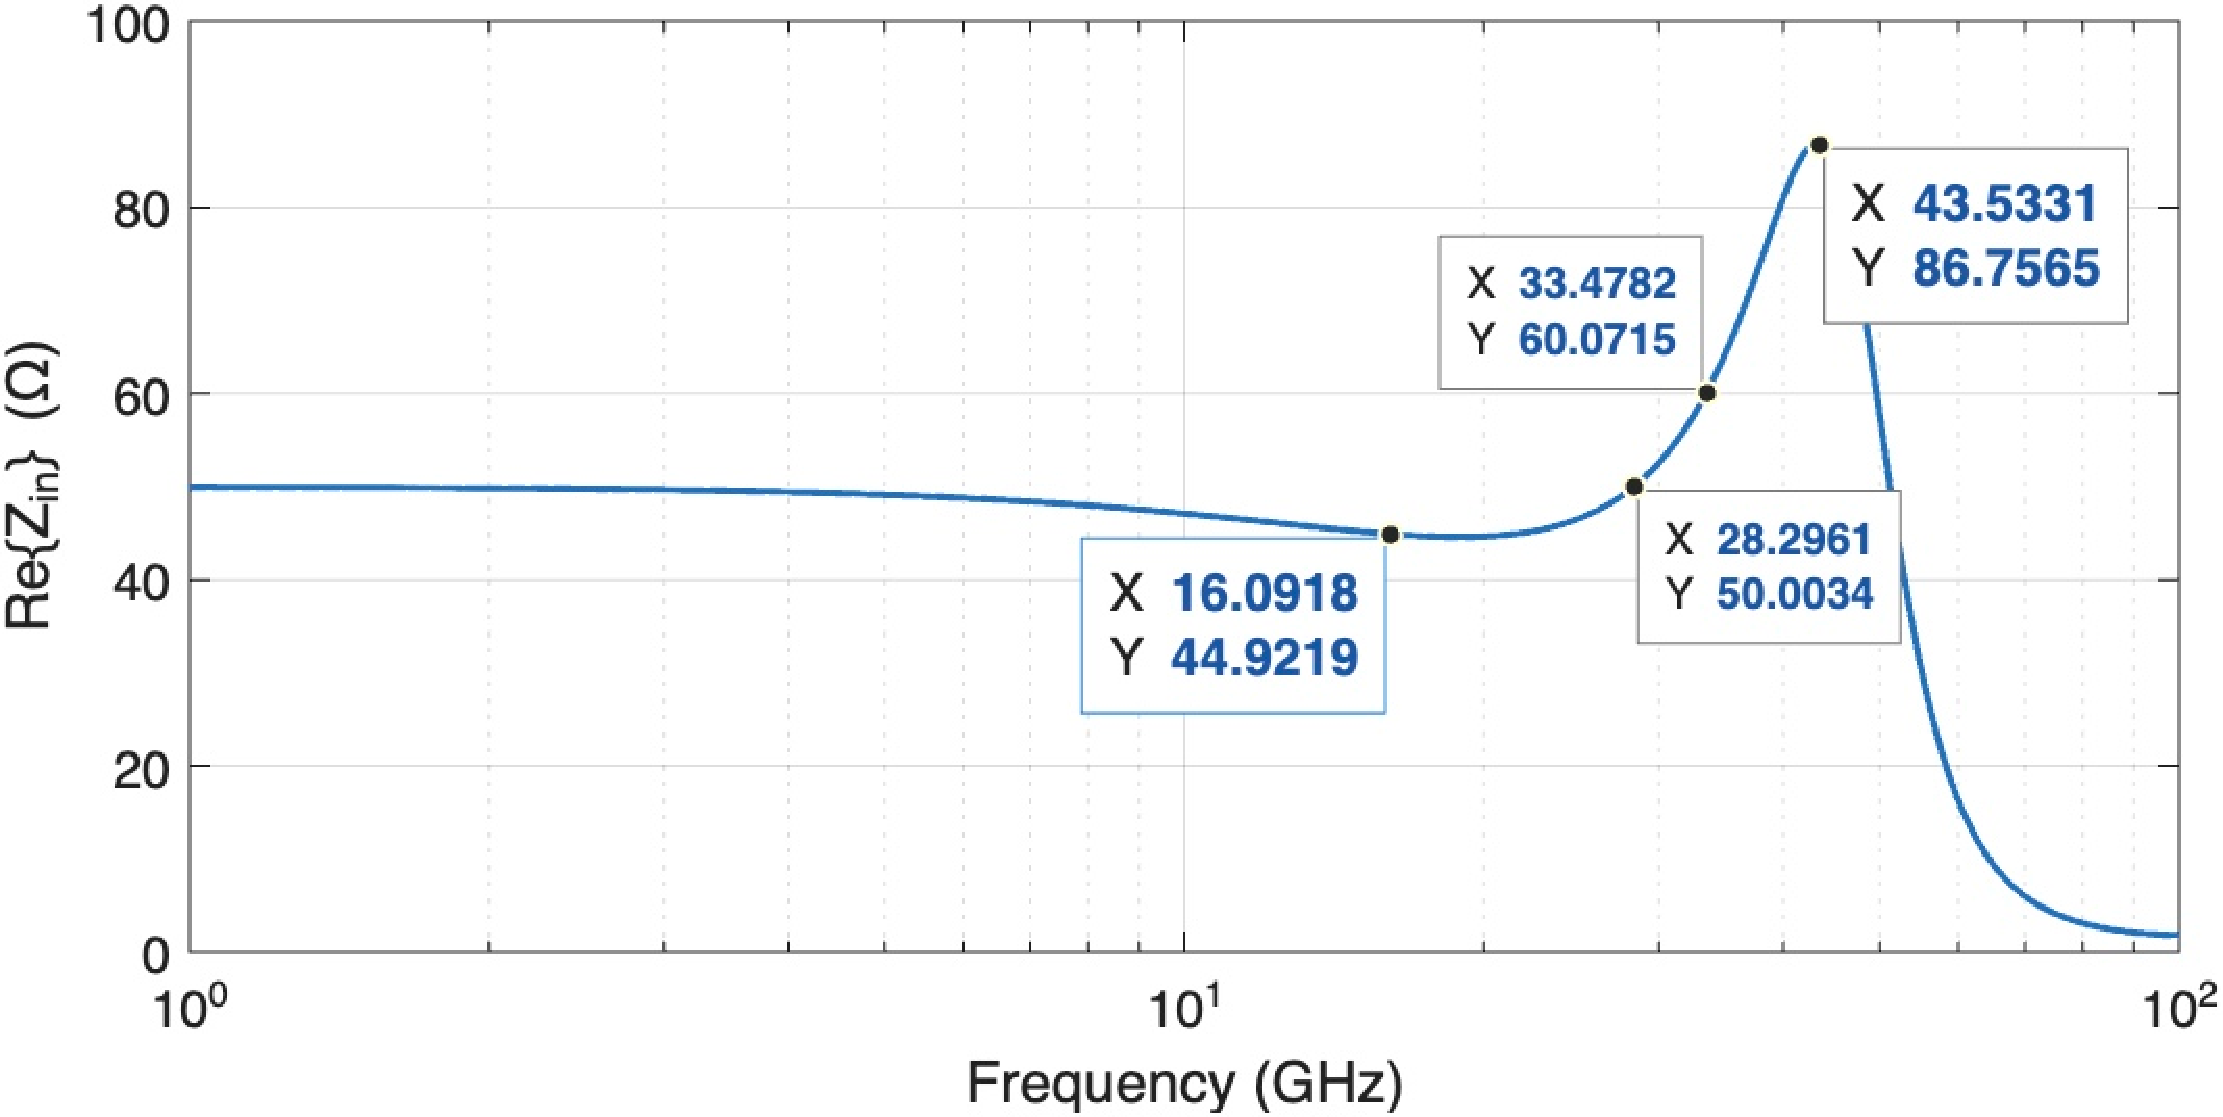
\includegraphics[width=\textwidth]{img/Termination_VGA_img/matlab_re_zin.pdf}
        \caption{Real input impedance, $\text{Re}\{Z_{in}\}$.}
        \label{fig:matlab_re}
    \end{subfigure}
    \hfill
    \begin{subfigure}[b]{0.48\textwidth}
        \centering
        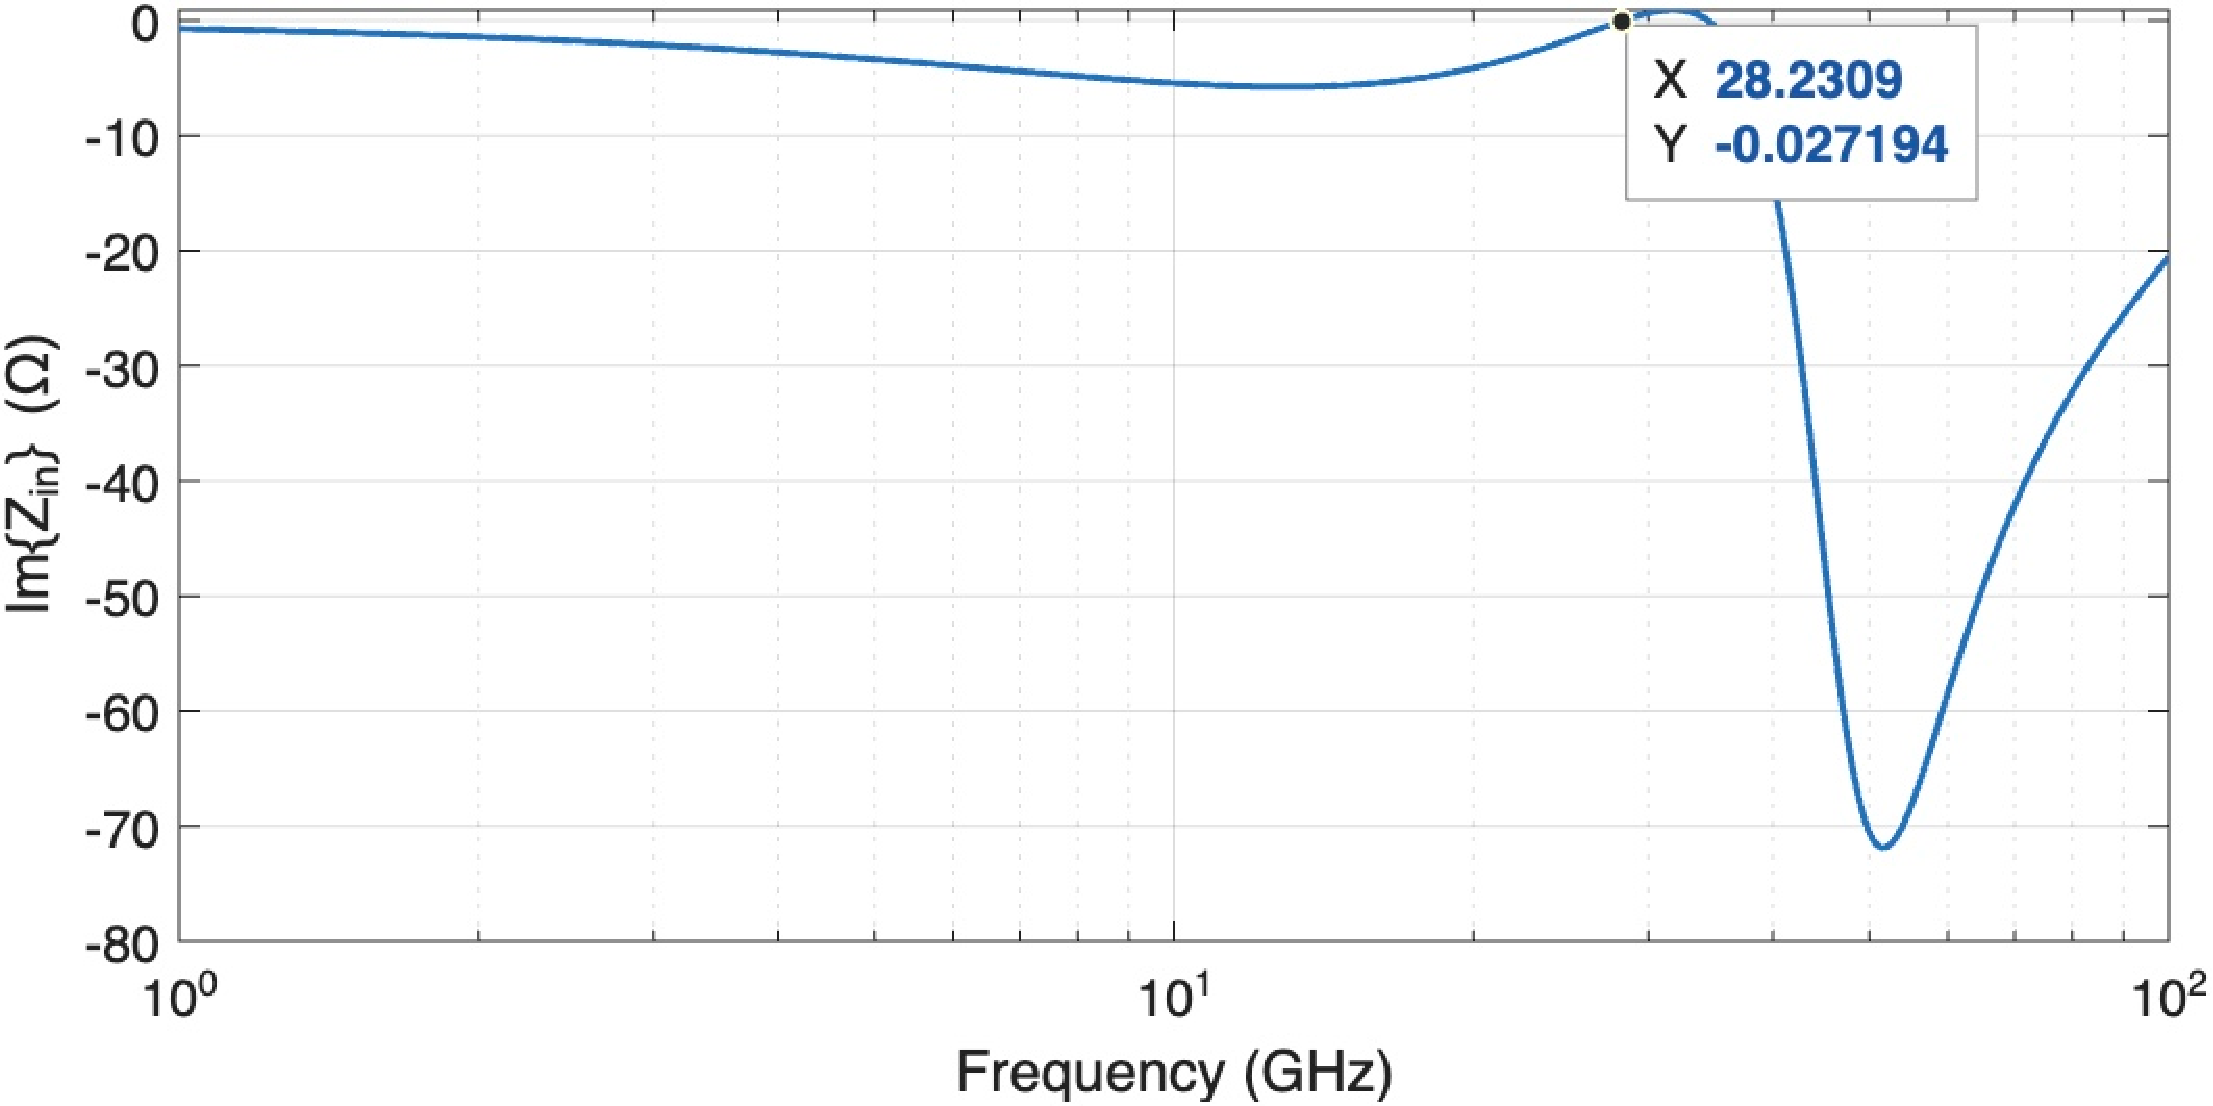
\includegraphics[width=\textwidth]{img/Termination_VGA_img/matlab_im_zin.pdf}
        \caption{Imaginary input impedance, $\text{Im}\{Z_{in}\}$.}
        \label{fig:matlab_im}
    \end{subfigure}

    \vspace{0.4cm} % Space between the top and bottom rows

    % --- Second Row ---
    \begin{subfigure}[b]{0.48\textwidth}
        \centering
        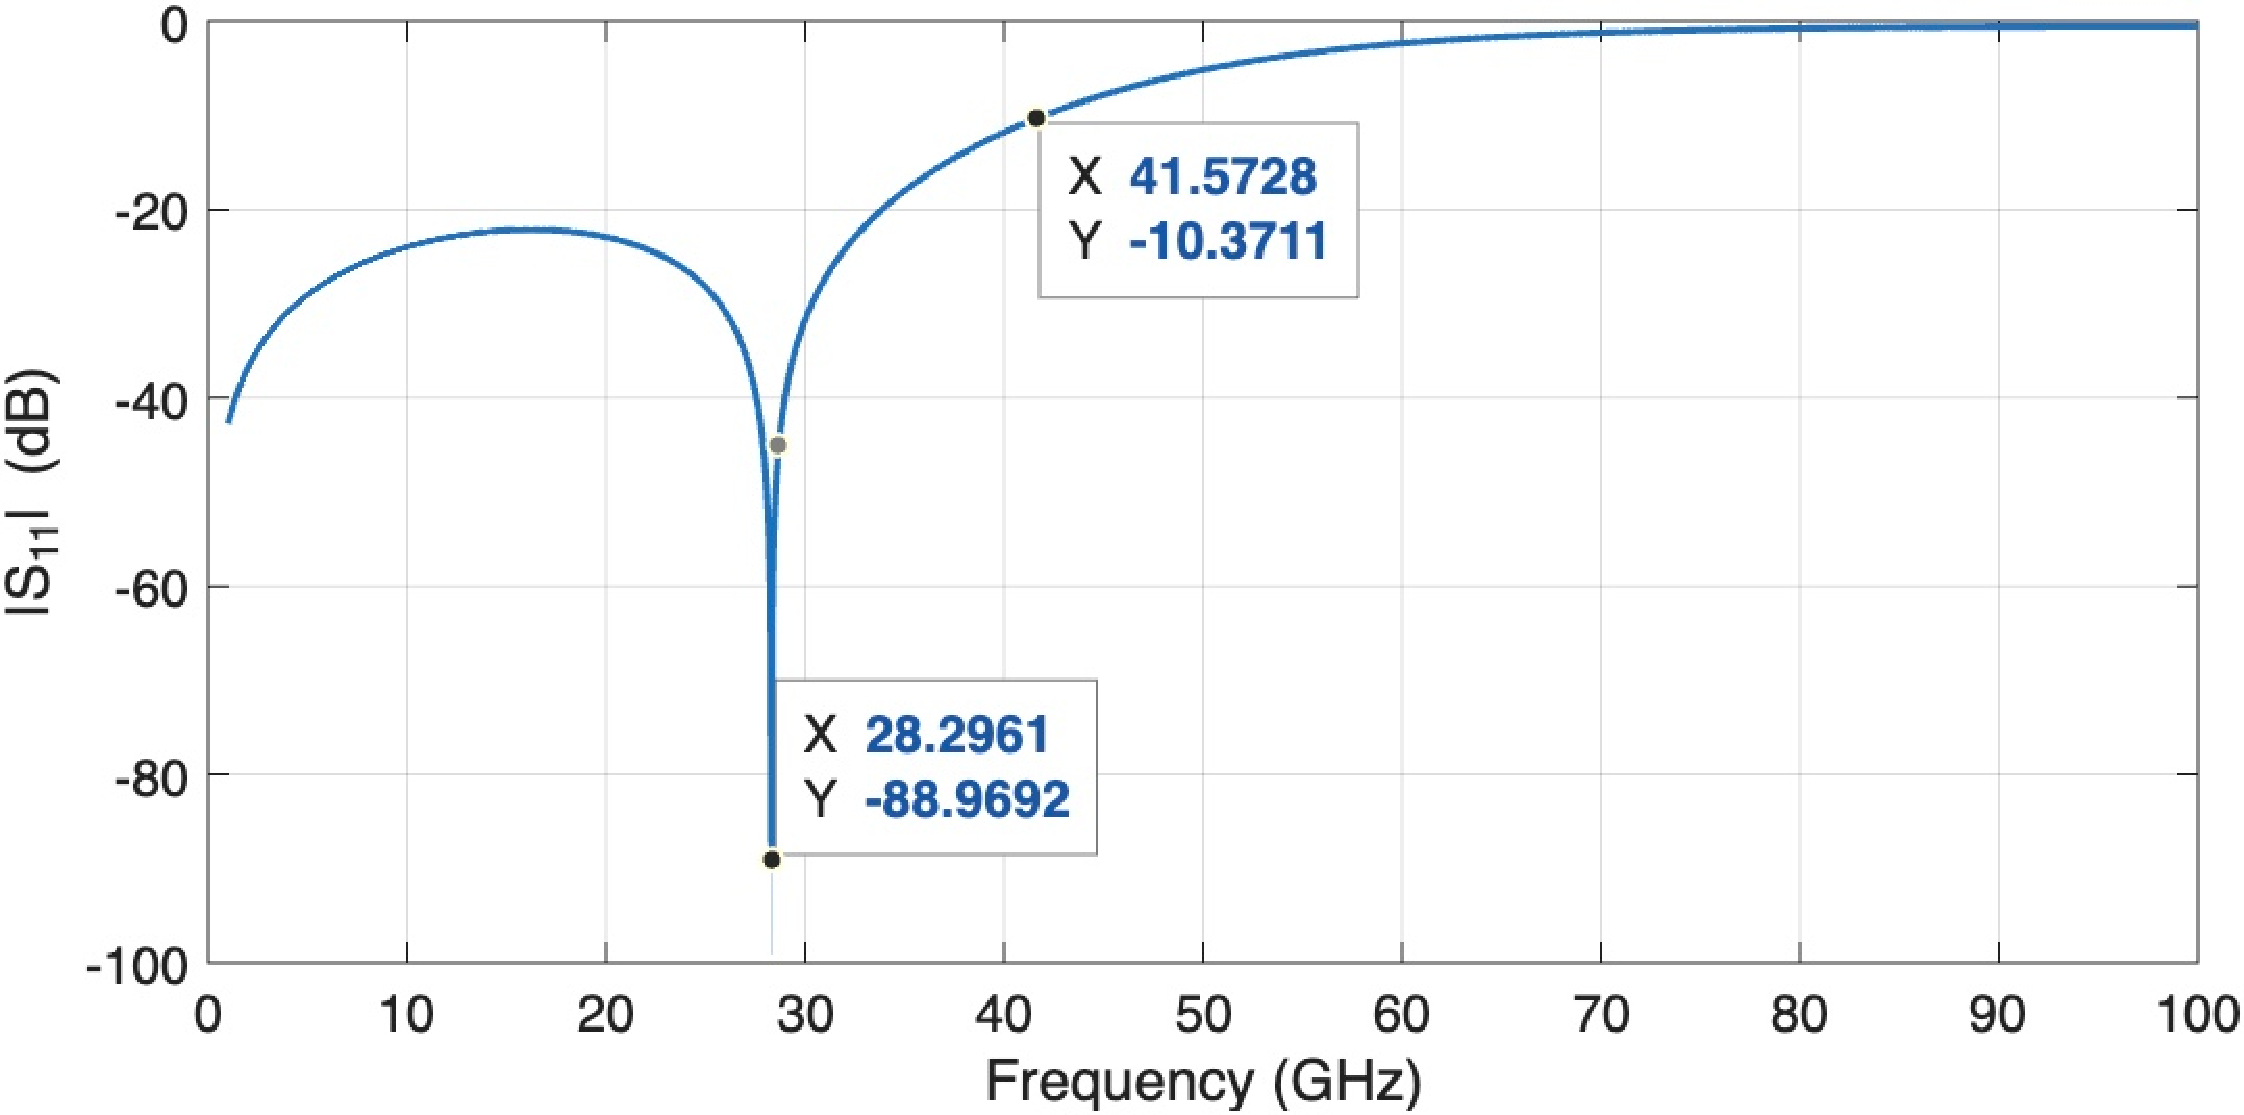
\includegraphics[width=\textwidth]{img/Termination_VGA_img/matlab_s11.pdf}
        \caption{Return loss $S_{11}$ (dB) referenced to $50\,\Omega$.}
        \label{fig:matlab_s11}
    \end{subfigure}
    \hfill
    \begin{subfigure}[b]{0.48\textwidth}
        \centering
        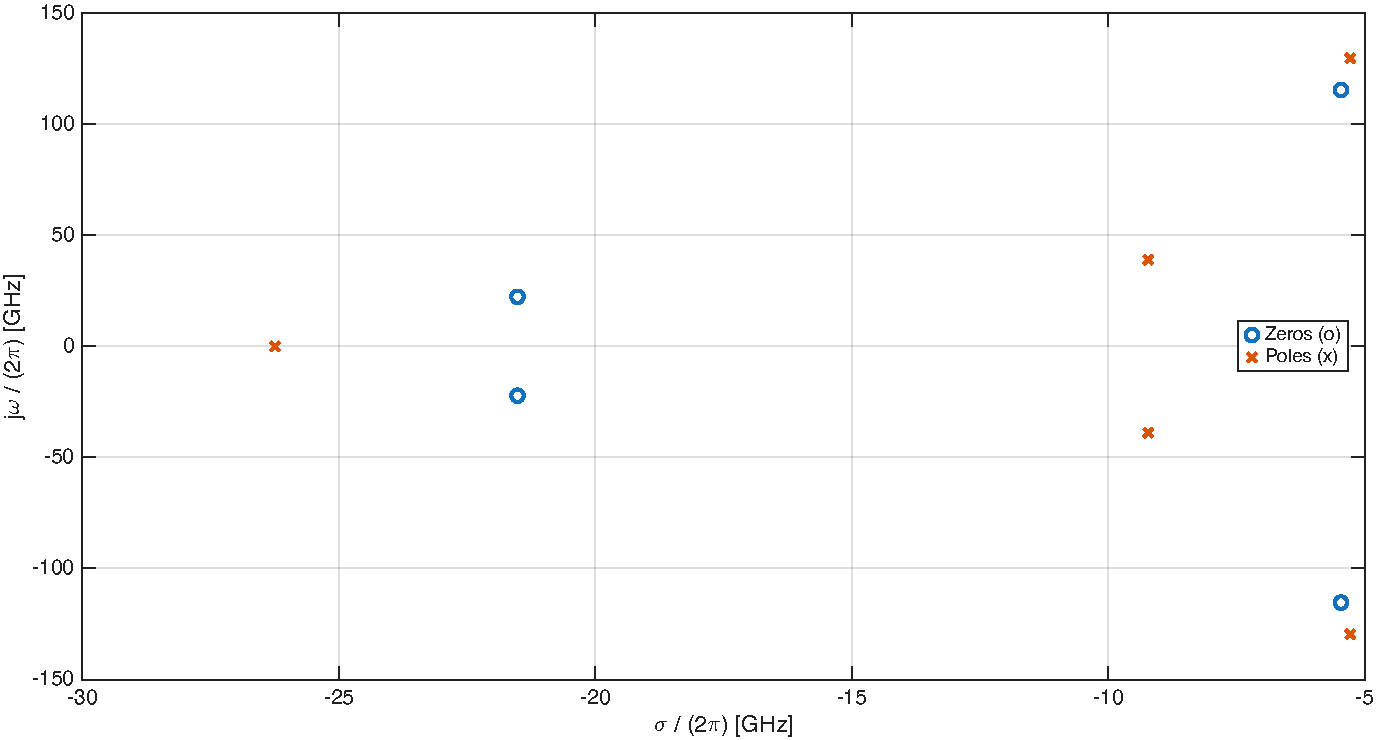
\includegraphics[width=\textwidth]{img/Termination_VGA_img/matlab_pz.pdf}
        \caption{Pole-zero map of $Z_{in}(s)$.}
        \label{fig:matlab_pz}
    \end{subfigure}

    \caption{Analytical MATLAB results for the optimised input network:
             $\text{Re}\{Z_{in}\}$, $\text{Im}\{Z_{in}\}$, $S_{11}$, and the pole-zero map.}
    \label{fig:matlab_analysis}
\end{figure}

% --- Target Values Table ---
\begin{table}[H]
    \centering
    \caption{Target component values}
    \label{tab:target_values}
    \begin{tabular}{@{}lc@{}}
        \toprule
        \textbf{Component Parameter} & \textbf{Target Value} \\
        \midrule
        Self-inductance ($L_1,\,L_2$)  & 130~pH  \\
        Coupling factor ($k$)           & $-0.4$  \\
        Bridging capacitance ($C_b$)    & 9.0~fF  \\
        \bottomrule
    \end{tabular}
\end{table}

% -------------------------------------------------------
\subsection{Proposed Topology}
% -------------------------------------------------------

\subsubsection*{Bridged-T Coil Bandwidth Extension}

A Bridged-T coil topology was selected to achieve the required broadband impedance match.
Unlike a simple series-peaking inductor, the symmetric T-coil exploits mutual coupling
between its two halves to split and absorb the parasitic capacitance of the ESD diode and
the receiver input gate, effectively distributing it across the network. The bridging
capacitor~$C_b$, connected across the outer terminals of the coil, provides an additional
high-frequency feed-forward current path that maintains the real impedance close to $50\,\Omega$
at the upper edge of the passband, where the inductors would otherwise present a high impedance.

\newpage
\subsubsection*{Digitally Controlled Impedance (DCI)}

Polysilicon resistors are subject to process and temperature (PT) variation of up to
$\pm 20\%$, which would cause a static resistor termination to drift well outside the
required $50\,\Omega$ window. To guarantee compliance across all corners, an active
Digitally Controlled Impedance (DCI) network was designed.

\vspace{\baselineskip}

The DCI employs a complementary topology: a PMOS pull-up network~($R_{UP}$) and an NMOS
pull-down network~($R_{Down}$) are connected in parallel between supply and ground at
the input node. This structure serves a dual purpose. First, the parallel combination of
the two branches sets the AC termination impedance seen by the channel:
\begin{equation}
    R_{Term} = \frac{R_{UP} \cdot R_{Down}}{R_{UP} + R_{Down}} = 50\,\Omega
    \label{eq:rterm}
\end{equation}
Second, the same resistive divider establishes the DC common-mode voltage at the input node:
\begin{equation}
    V_{CM} = V_{DD} \cdot \frac{R_{Down}}{R_{UP} + R_{Down}}
    \label{eq:vcm}
\end{equation}
Solving Equations~\eqref{eq:rterm} and~\eqref{eq:vcm} simultaneously for the target
$V_{CM} = 540\,\text{mV}$ and $V_{DD} = 0.9\,\text{V}$ yields $R_{UP} = 74.1\,\Omega$
and $R_{Down} = 153.8\,\Omega$.

\vspace{\baselineskip}

To counter PT variation, each branch implements a 4-bit binary-weighted tuning array.
An always-on base leg is sized to achieve the target resistance at the fastest (FF) process
corner, where resistors are at their minimum value. For slower corners, the four binary
tuning legs add parallel conductance in discrete steps. The target resistance of each
tuning branch follows a binary scaling law:
\begin{equation}
    R_{branch,\,n} = \frac{R_{branch,\,0}}{2^{n}}, \quad n = 0, 1, 2, 3
    \label{eq:rbranch}
\end{equation}
Because each tuning switch contributes a finite ON-resistance ($R_{SW}$), the physical
polysilicon resistor drawn in layout is reduced by that amount to preserve the target
branch resistance:
\begin{equation}
    R_{Drawn} = R_{branch,\,n} - R_{SW}
    \label{eq:rdrawn}
\end{equation}

The schematic of the proposed input network topology is shown in
Figure~\ref{fig:input_schematic}, and the full DCI circuit implementation is shown in
Figure~\ref{fig:dci_schematic}.

\begin{figure}[H]
    \centering
    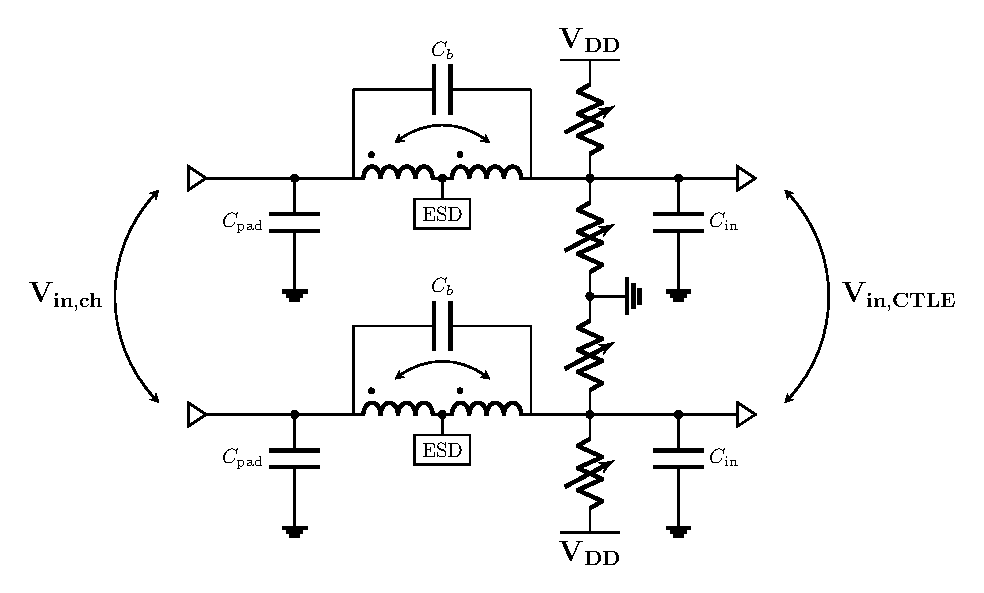
\includegraphics[width=0.75\textwidth]{img/Termination_VGA_img/input_network_sch.pdf}
    \caption{Proposed Bridged-T input network schematic, showing the differential
             T-coil pair, ESD protection, $C_b$, $C_{in}$, and the DCI termination.}
    \label{fig:input_schematic}
\end{figure}

\begin{figure}[H]
    \centering
    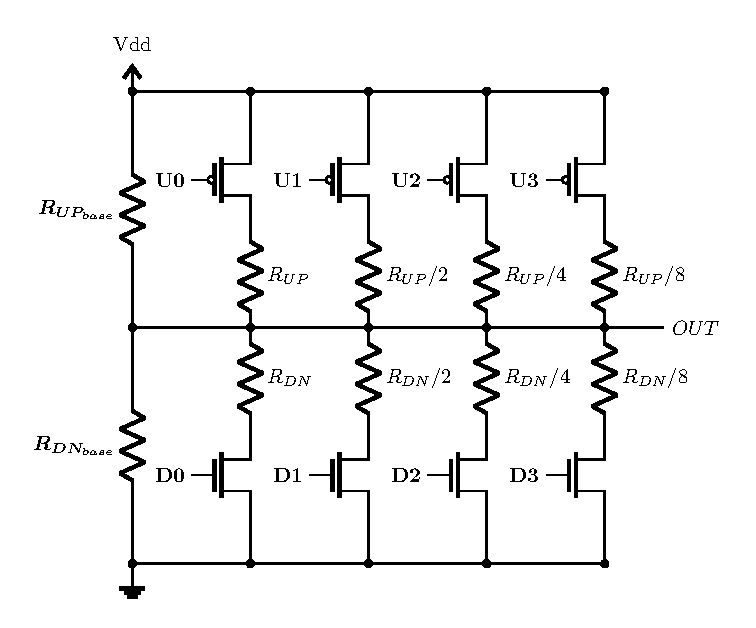
\includegraphics[width=0.7\textwidth]{img/Termination_VGA_img/DCI_sch.pdf}
    \caption{Complementary PMOS/NMOS Digitally Controlled Impedance (DCI)
             circuit, showing the always-on base leg and the four binary tuning branches.}
    \label{fig:dci_schematic}
\end{figure}

% -------------------------------------------------------
\subsection{Implementation and Simulation Results}
% -------------------------------------------------------

\subsubsection{T-Coil Design and EMX Extraction}

The T-coil was implemented as an octagonal symmetric spiral on the thick top metal layers to
maximise the quality factor~$Q$. The geometry was iteratively optimised in EMX to simultaneously
meet the self-inductance and coupling factor targets derived from the analytical model.
The extracted frequency-dependent parameters are plotted in Figure~\ref{fig:tcoil_emx_full},
and the physical layout dimensions together with the achieved parasitic values are
summarised in Tables~\ref{tab:tcoil_dims} and~\ref{tab:achieved_values} respectively.

% --- T-coil EMX results: 2x2 grid ---
\begin{figure}[H]
    \centering
    \begin{subfigure}[b]{0.48\textwidth}
        \centering
        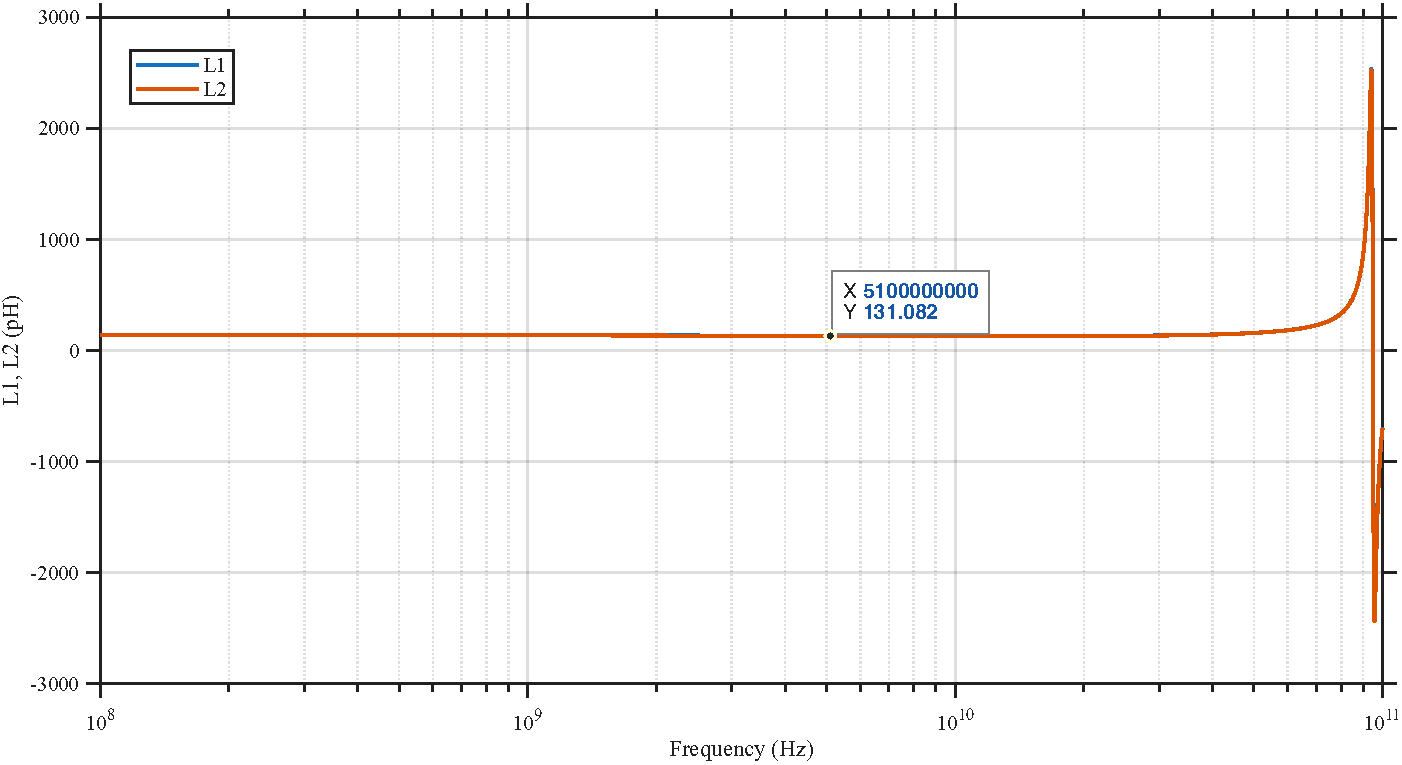
\includegraphics[width=\textwidth]{img/Termination_VGA_img/tcoil_L.pdf}
        \caption{Self-inductance $L_1,\,L_2$ vs.\ frequency.}
        \label{fig:tcoil_L}
    \end{subfigure}
    \hfill
    \begin{subfigure}[b]{0.48\textwidth}
        \centering
        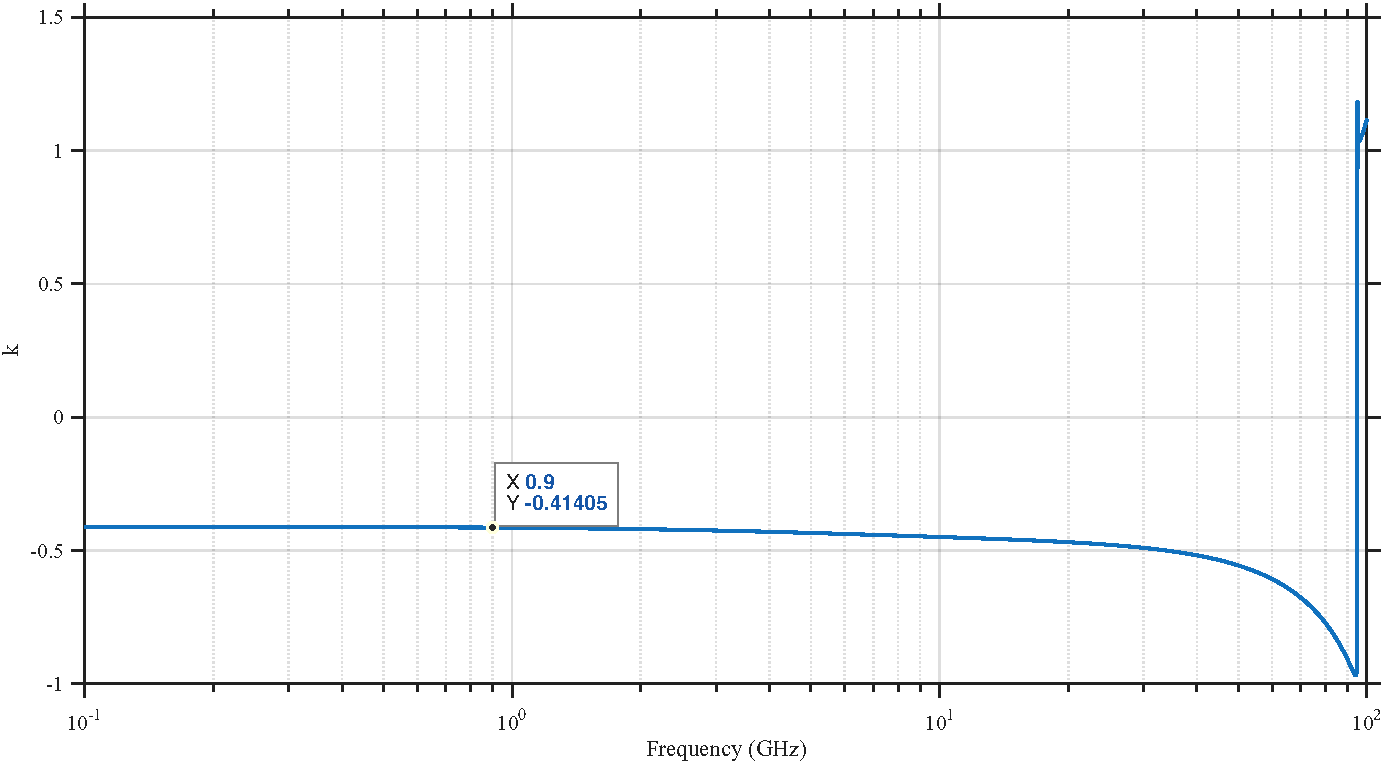
\includegraphics[width=\textwidth]{img/Termination_VGA_img/tcoil_k.pdf}
        \caption{Coupling factor $k$ vs.\ frequency.}
        \label{fig:tcoil_k}
    \end{subfigure}

    \vspace{10pt}

    \begin{subfigure}[b]{0.48\textwidth}
        \centering
        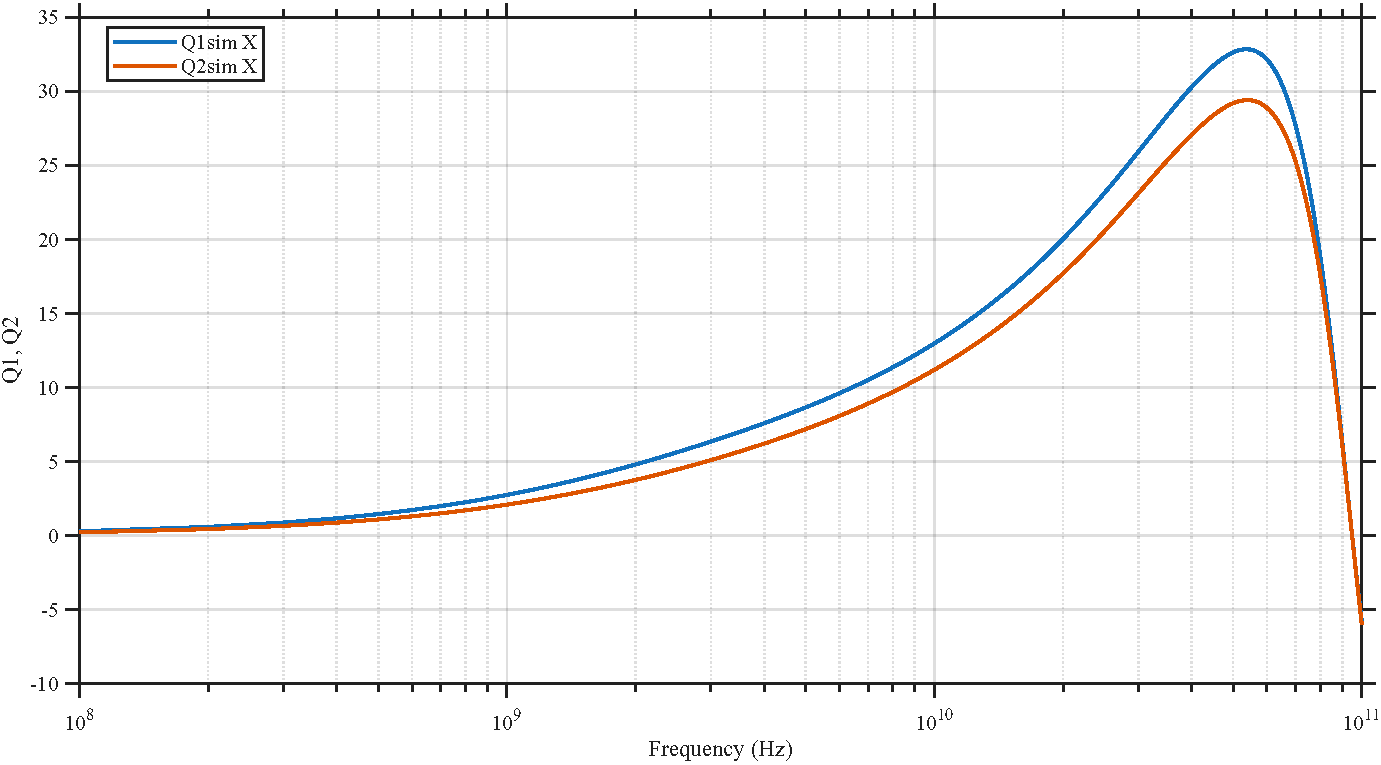
\includegraphics[width=\textwidth]{img/Termination_VGA_img/tcoil_Q.pdf}
        \caption{Quality factor $Q$ vs.\ frequency.}
        \label{fig:tcoil_Q}
    \end{subfigure}
    \hfill
    \begin{subfigure}[b]{0.48\textwidth}
        \centering
        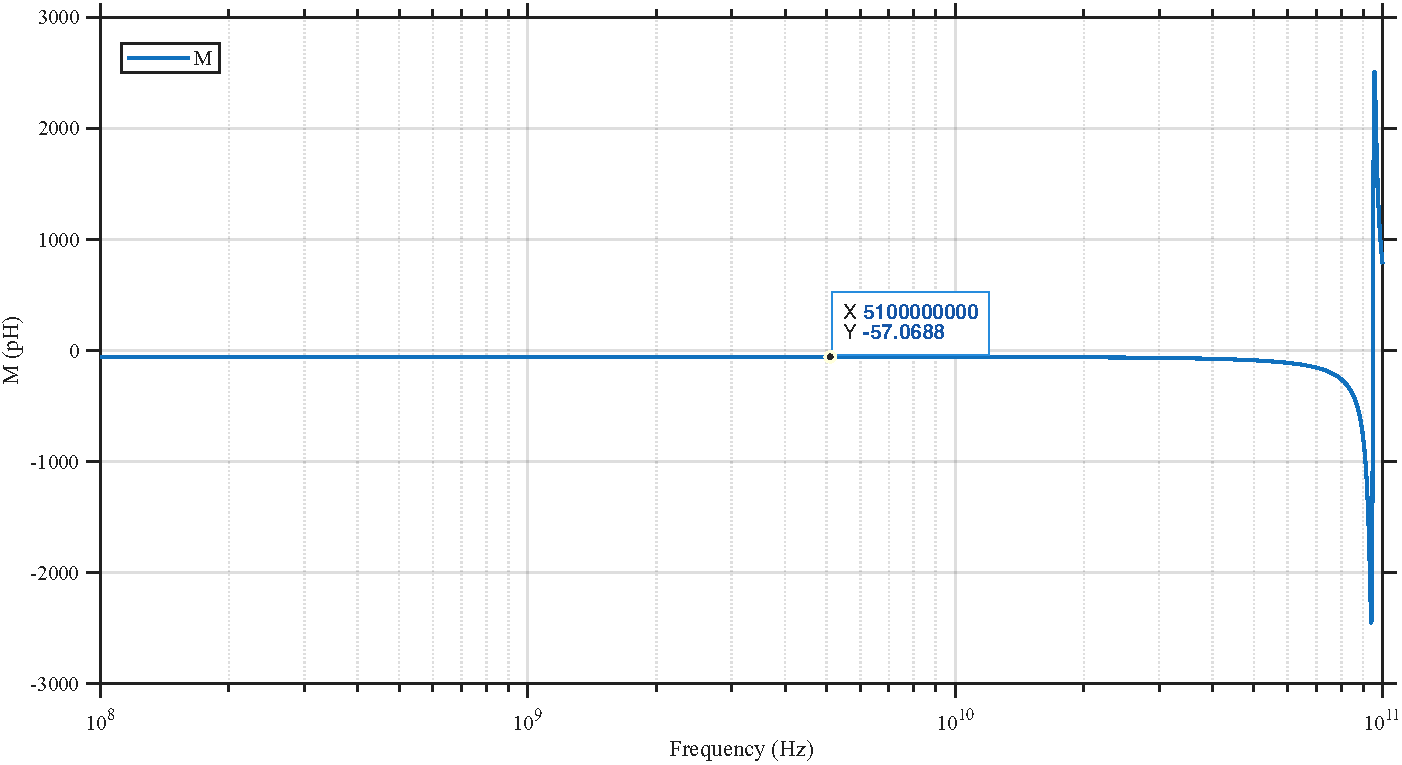
\includegraphics[width=\textwidth]{img/Termination_VGA_img/tcoil_M.pdf}
        \caption{Mutual inductance $M$ vs.\ frequency.}
        \label{fig:tcoil_M}
    \end{subfigure}

    \caption{EMX post-layout simulation results for the T-coil: self-inductance,
             coupling factor, quality factor, and mutual inductance across frequency.}
    \label{fig:tcoil_emx_full}
\end{figure}

\begin{figure}[H]
    \centering
    % --- Left side: The Layout Figure ---
    \begin{minipage}[c]{0.45\textwidth}
        \centering
        % \textwidth here refers to the width of the minipage
        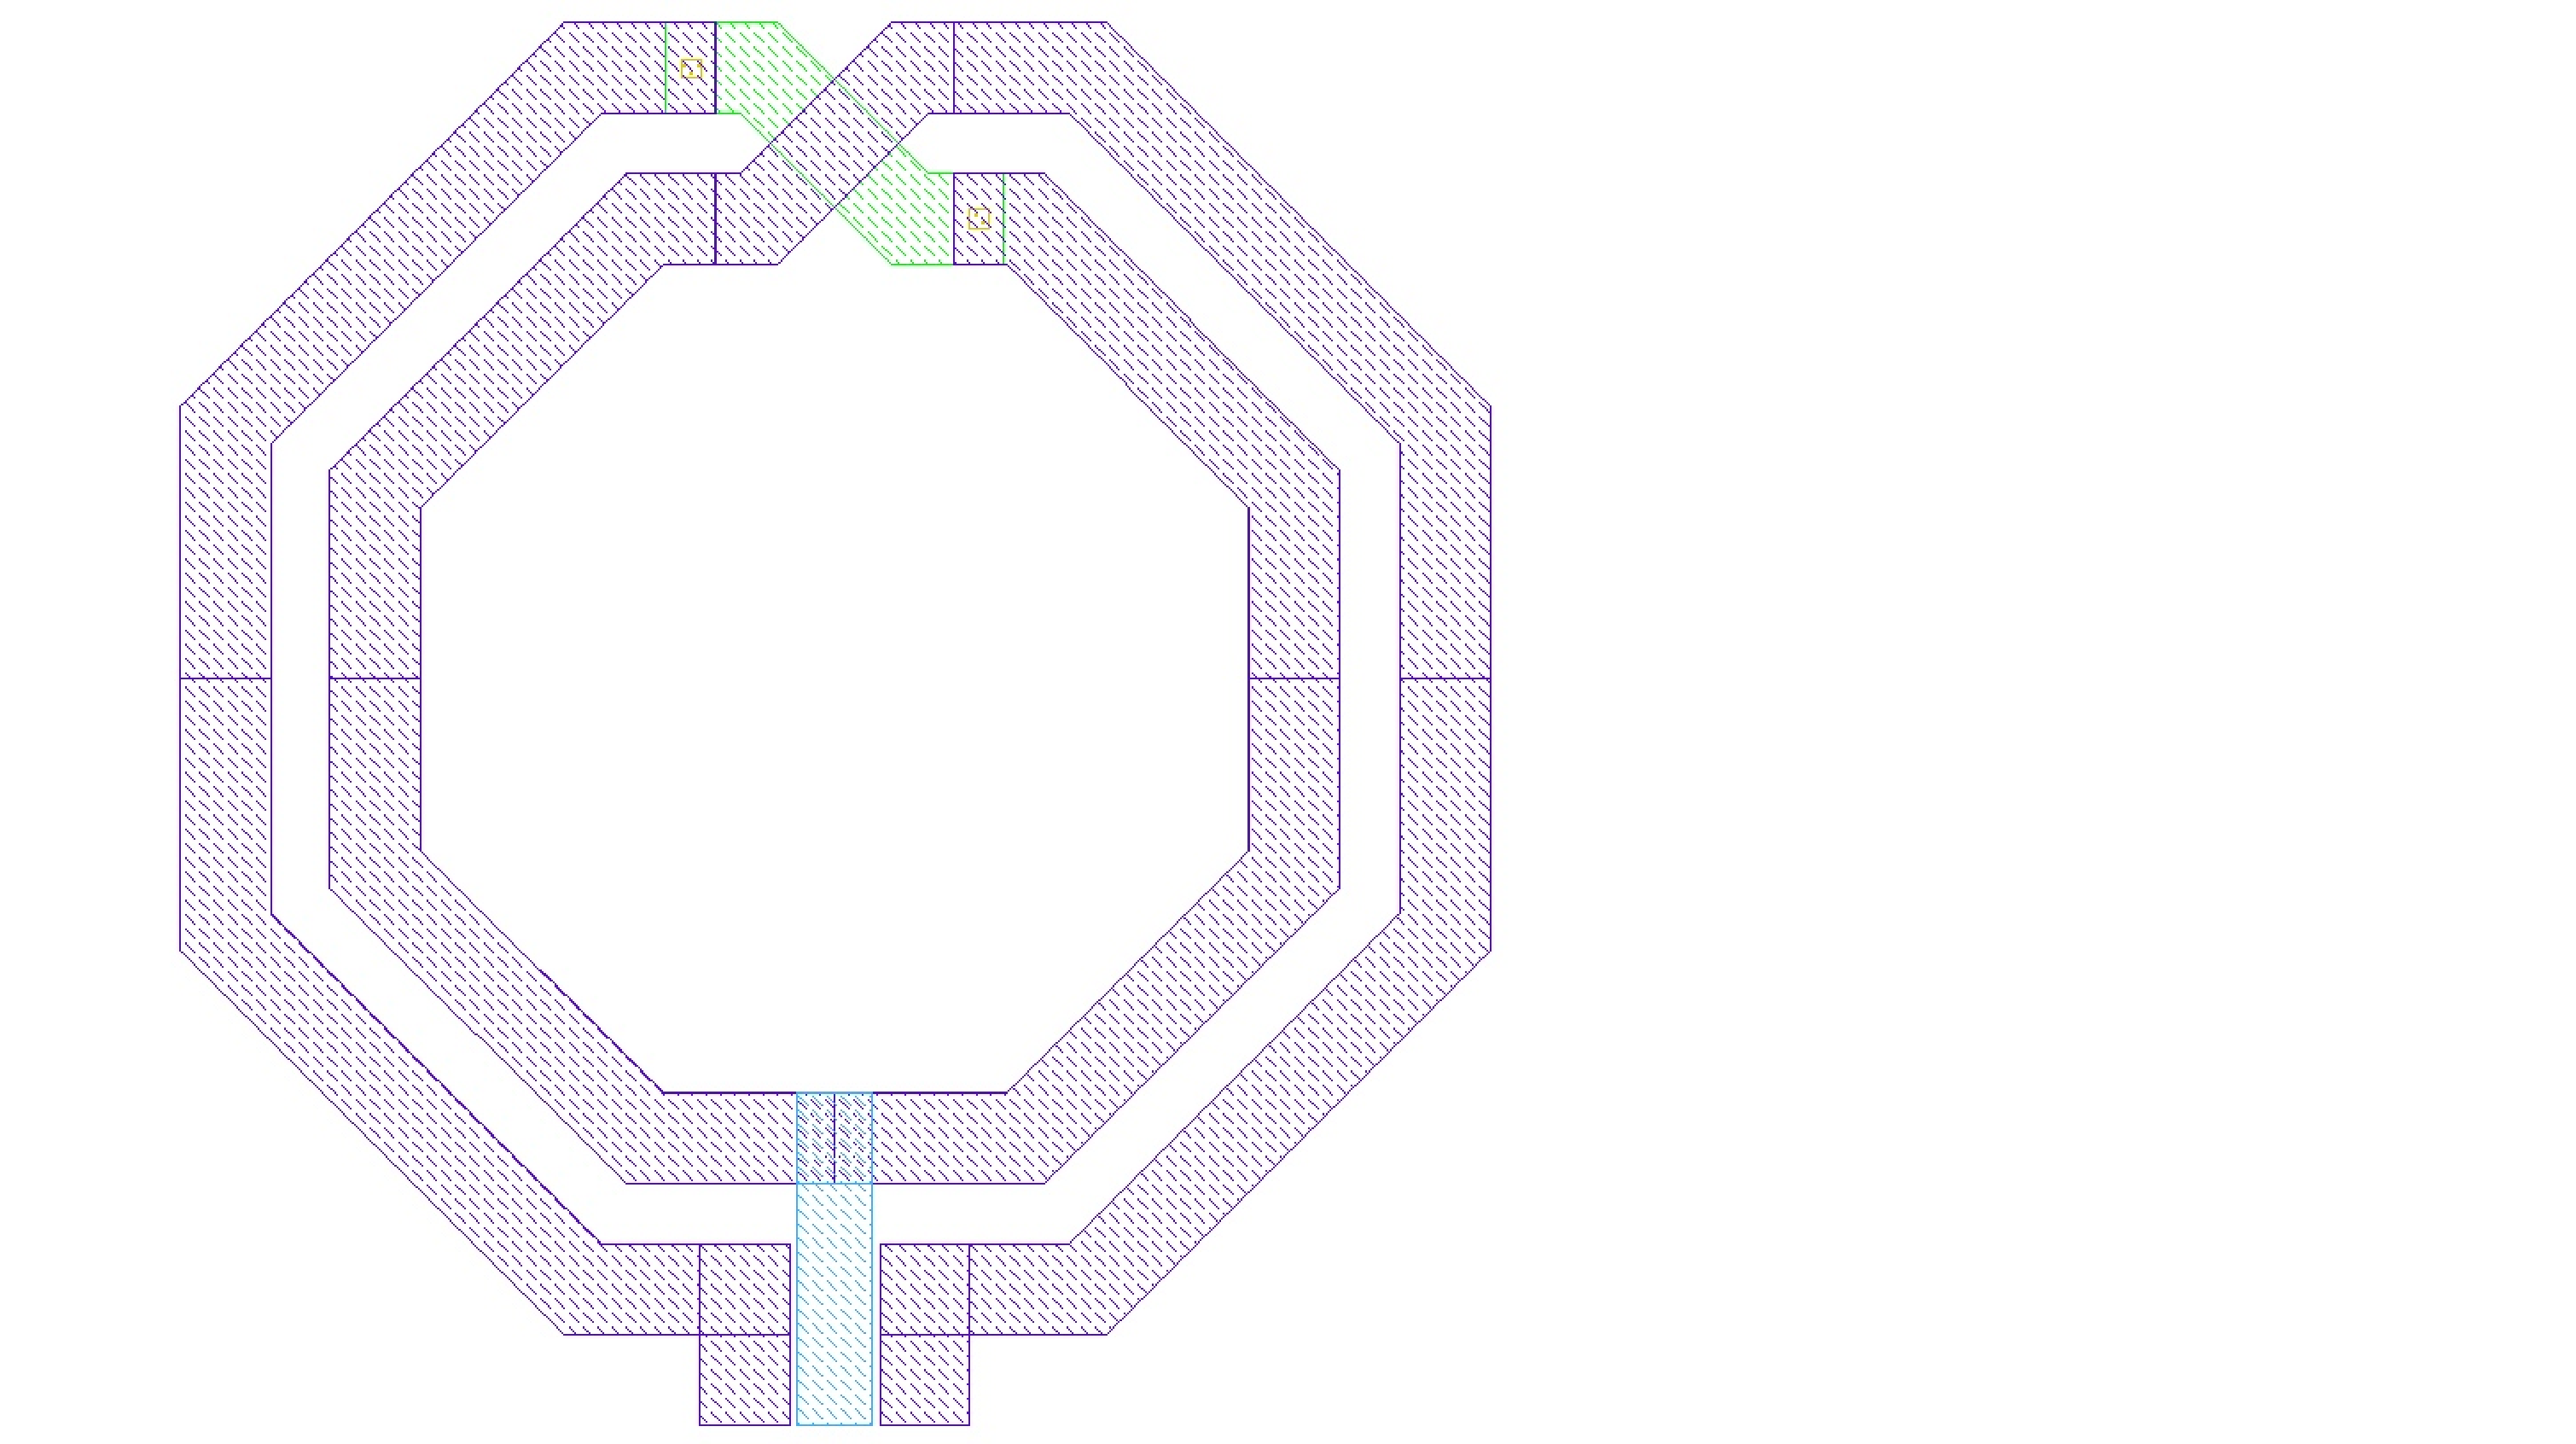
\includegraphics[width=0.7\textwidth]{img/Termination_VGA_img/tcoil_layout.pdf}
        \caption{Octagonal T-coil layout.}
        \label{fig:tcoil_layout}
    \end{minipage}\hfill
    % --- Right side: The Dimensions Table ---
    \begin{minipage}[c]{0.45\textwidth}
        \centering
        \captionof{table}{T-Coil Physical Dimensions}
        \label{tab:tcoil_dims}
        \begin{tabular}{@{}ll@{}}
            \toprule
            \textbf{Parameter}          & \textbf{Value}     \\
            \midrule
            Outer diameter ($OD$)       & $87\,\mu\text{m}$  \\
            Inner diameter ($ID$)       & $55\,\mu\text{m}$  \\
            Trace width ($W$)           & $6\,\mu\text{m}$   \\
            Turn spacing ($S$)          & $4\,\mu\text{m}$   \\
            Number of turns ($N$)       & 2                  \\
            \bottomrule
        \end{tabular}
    \end{minipage}
\end{figure}

\begin{table}[H]
    \centering
    \caption{T-coil parameters extracted from EMX}
    \label{tab:achieved_values}
    \begin{tabular}{@{}lcc@{}}
        \toprule
        \textbf{Parameter}              & \textbf{Target} & \textbf{Achieved (EMX)} \\
        \midrule
        Self-inductance ($L_1,\,L_2$)   & 130~pH          & 131~pH                  \\
        Coupling factor ($k$)           & $-0.4$          & $-0.41$                 \\
        \bottomrule
    \end{tabular}
\end{table}

\subsubsection{DCI Performance Across Corners}

The robustness of the DCI performance was evaluated across extreme process and temperature corners. As summarized in Table~\ref{tab:vcm_corners}, the output common-mode voltage ($V_{CM}$) exhibits exceptional stability. Thanks to the calibration framework, the total $V_{CM}$ deviation is tightly constrained to within $\pm 1\,\text{mV}$ of the nominal target across all simulated conditions. Furthermore, the 4-bit tuning array successfully regulates the input impedance, maintaining the nominal $50\,\Omega$ termination with a maximum worst-case variation of less than $4\,\Omega$.

\begin{table}[H]
    \centering
    \caption{Common-mode voltage ($V_{CM}$) and termination stability across PVT corners}
    \label{tab:vcm_corners}
    \begin{tabular}{@{}lccccc@{}}
        \toprule
        \textbf{Parameter} & \textbf{Nominal} & \textbf{SS, $125^\circ$C} & \textbf{SS, $-40^\circ$C} & \textbf{FF, $125^\circ$C} & \textbf{FF, $-40^\circ$C} \\
        \midrule
        $V_{CM}$ (mV) & 540.9 & 541.5 & 540.7 & 540.3 & 541.4 \\
        $R_{Term}$ ($\Omega$) & 49.87 & 53.56 & 52.11 & 50.58 & 49.86 \\
        \bottomrule
    \end{tabular}
\end{table}

% -------------------------------------------------------
\subsubsection{Complete Input Network Testbench}
% -------------------------------------------------------
 
The full top-level simulation was conducted using the differential testbench illustrated in Figure~\ref{fig:full_tb}. The architecture consists of two identical single-ended input network instances configured differentially. Each half-circuit integrates the fully extracted post-layout T-coil, the DCI termination network, and lumped models representing the front-end parasitic capacitances ($C_{pad} = 50\,\text{fF}$, $C_{ESD} = 60\,\text{fF}$, and $C_{in} = 35\,\text{fF}$).

In accordance with PCI-SIG specifications, a $265\,\text{nF}$ AC coupling capacitor ($C_c$) is placed in series with the input port. Its impedance is negligible at high frequencies ($|Z_{C_c}| < 1\,\text{m}\Omega$ at $1\,\text{GHz}$), ensuring it does not affect the AC response. Its primary purpose is to provide required DC isolation by blocking the $540\,\text{mV}$ DCI common-mode bias from reaching the $50\,\Omega$ measurement port.

The DCI digital interface is driven by a custom Verilog-A behavioral decoder (\texttt{DCIctrl}). This block translates a single parametric DC voltage into the 4-bit binary control code (UP$\langle$3:0$\rangle$ and DN$\langle$3:0$\rangle$) required to tune the termination matrix.

\begin{figure}[H]
    \centering
    \framebox{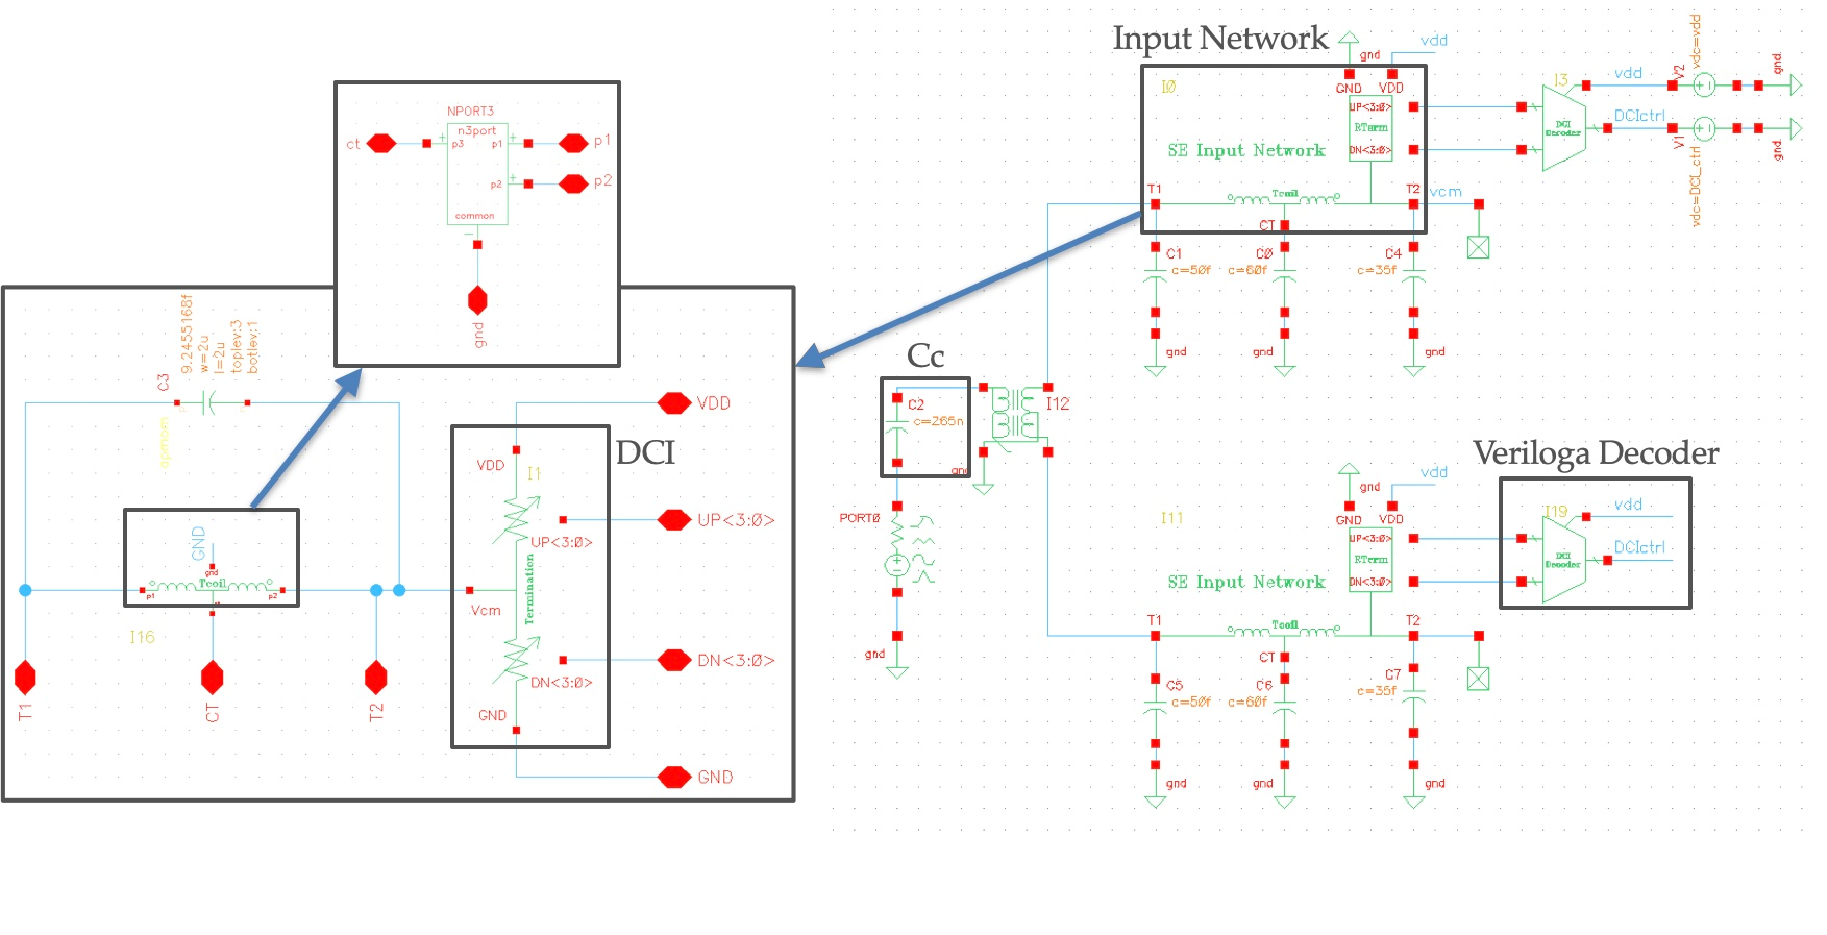
\includegraphics[width=0.95\textwidth]{img/Termination_VGA_img/testbenchinput.pdf}}
    \caption{Differential input network simulation testbench.}
    \label{fig:full_tb}
\end{figure}

\subsubsection{Overall Input Network Performance}
As illustrated in Figure~\ref{fig:overall_perf}, the input network exhibits broadband matching performance that significantly exceeds the PCI-SIG compliance mask. The standard dictates a differential return loss ($S_{11}$) strictly below $-10\,\text{dB}$ up to $1.25\,\text{GHz}$, relaxing to $-8\,\text{dB}$ up to $16\,\text{GHz}$. In contrast, the proposed design effortlessly maintains an $S_{11}$ below $-10\,\text{dB}$ across an extended bandwidth up to $35\,\text{GHz}$. Furthermore, the real input impedance ($R_{in}$) remains tightly bounded between $40\,\Omega$ and $60\,\Omega$ up to $25\,\text{GHz}$, ensuring robust signal integrity.

% --- Overall performance: stacked 2x1 ---
\begin{figure}[H]
    \centering

    \begin{subfigure}[b]{0.9\textwidth}
        \centering
        \framebox{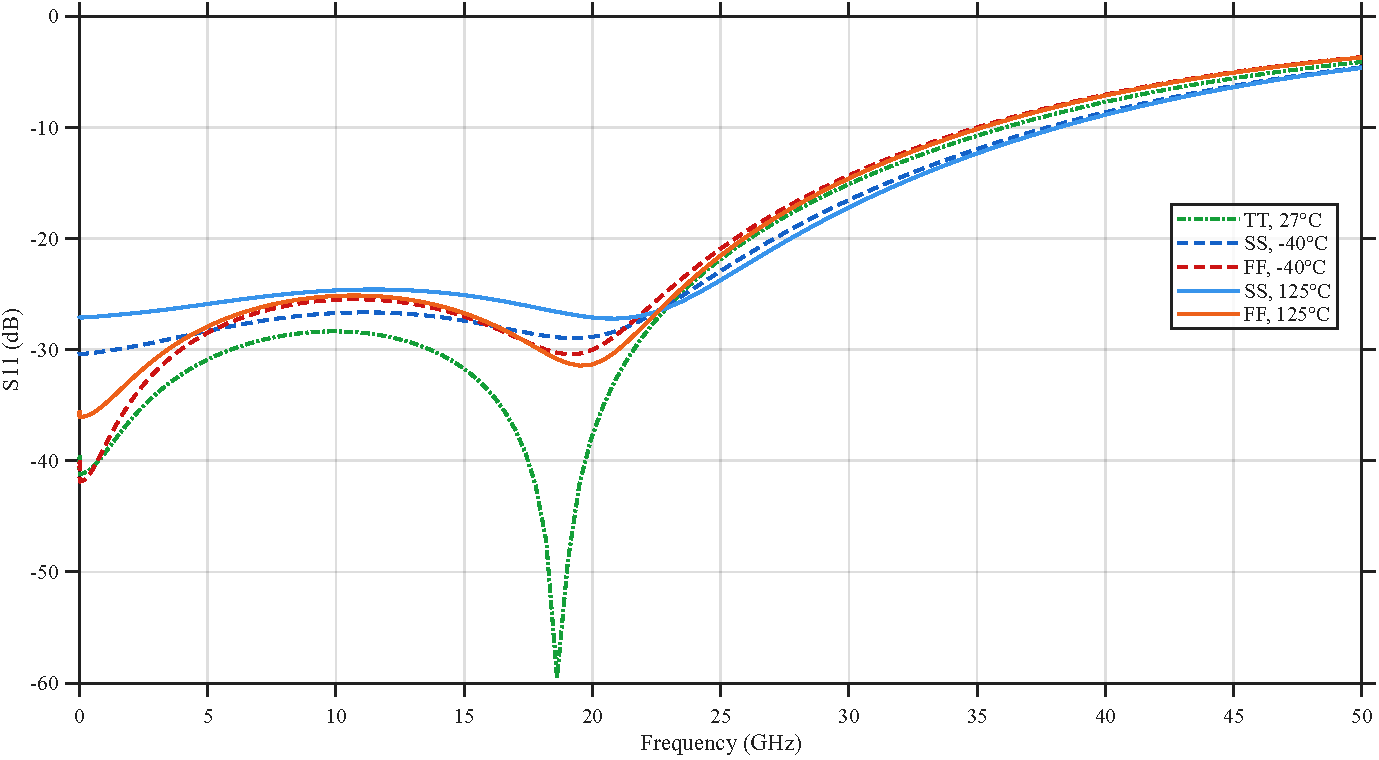
\includegraphics[width=\textwidth]{img/Termination_VGA_img/in_S11.pdf}}
        \caption{Overall Input Network $S_{11}$}
        \label{fig:overall_s11}
    \end{subfigure}

    \vspace{1cm}

    \begin{subfigure}[b]{0.9\textwidth}
        \centering
        \framebox{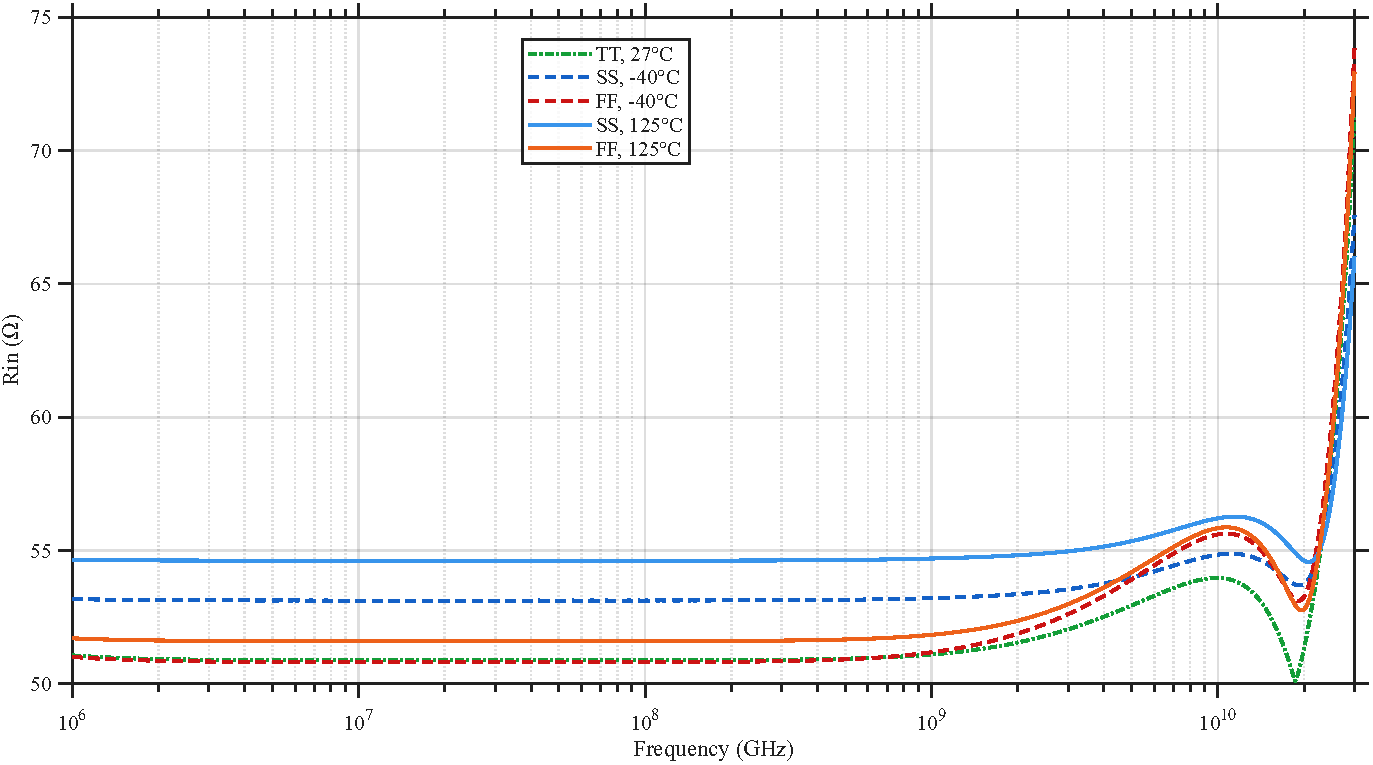
\includegraphics[width=.95\textwidth]{img/Termination_VGA_img/in_Rin.pdf}}
        \caption{Overall Real Input Impedance $R_{in}$}
        \label{fig:overall_rin}
    \end{subfigure}

    \caption{Top-level AC performance of the complete receiver input network.}
    \label{fig:overall_perf}
\end{figure}
